\section{Triangle-Feed Antenna}

A prototype of the triangle-feed antenna has been built. The results will be described in this section.

The prototype is shown in Figure~\ref{fig:triang_proto}. Compared to the simulation, see Figure~\ref{fig:ant2techschem}, a \SI{5}{mm} strip of copper has been added next to the feed line.  \fixme{Simulation results when adding this copper strip. Describe why this works.}

\begin{figure}[htbp]
    \centering
    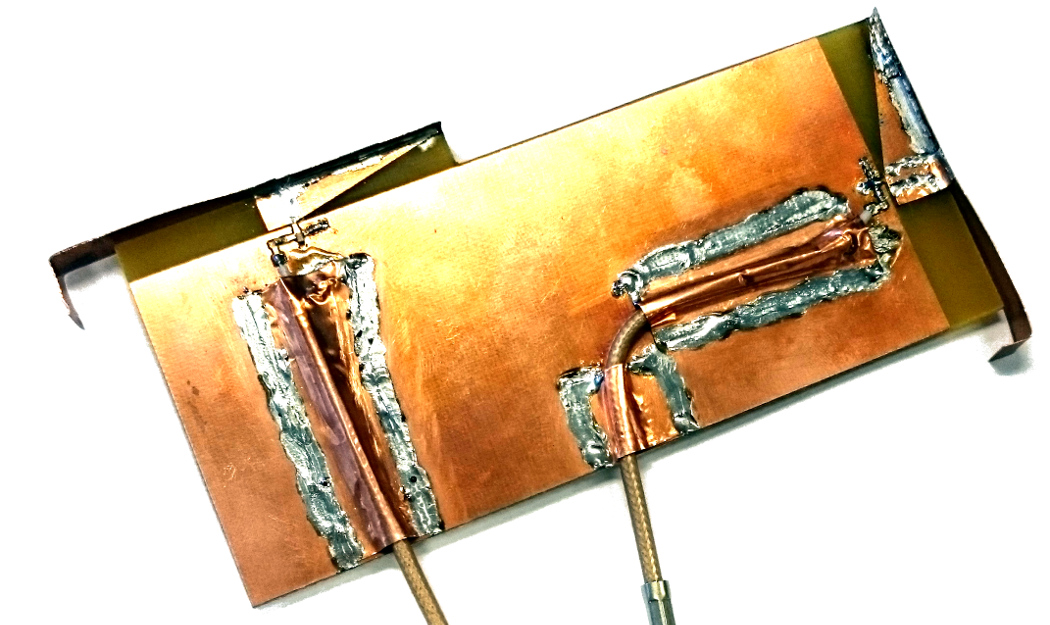
\includegraphics{img/tech_sol/trianglefeed/mockup/mockup.jpg}
    \caption{Triangle-feed antenna prototype.}
    \label{fig:triang_proto}
\end{figure}

The antenna has initially been matched for the best bandwidth. The component values are shown in Figure~\ref{fig:triang_proto_matching}.

\begin{figure}[htbp]
        \centering
        \begin{tabular}{m{3in}m{3in}}
            \centering
            \includegraphics{img/tech_sol/schematic_tuning_1}&
            \centering
            \footnotesize
            \begin{tabular}{|l|l|l|l|}
                \hline
                & $C_1$ & $L_1$ & $C_2$ \\
                \hline
                Top antenna & \SI{3.0}{pF} & \SI{6.8}{nH} & \SI{0.9}{pF} \\
                Side antenna & \SI{2.2}{pF} & \SI{5.6}{nH} & \SI{0.3}{pF} \\
                \hline
            \end{tabular}
        \end{tabular}
    \caption{Matching circuit for the triangle-feed antenna prototype. These are the component values where the bandwidth is found to be the largest.}
    \label{fig:triang_proto_matching}
\end{figure}
